\documentclass[man,floatsintext]{apa6}
\usepackage{lmodern}
\usepackage{amssymb,amsmath}
\usepackage{ifxetex,ifluatex}
\usepackage{fixltx2e} % provides \textsubscript
\ifnum 0\ifxetex 1\fi\ifluatex 1\fi=0 % if pdftex
  \usepackage[T1]{fontenc}
  \usepackage[utf8]{inputenc}
\else % if luatex or xelatex
  \ifxetex
    \usepackage{mathspec}
  \else
    \usepackage{fontspec}
  \fi
  \defaultfontfeatures{Ligatures=TeX,Scale=MatchLowercase}
\fi
% use upquote if available, for straight quotes in verbatim environments
\IfFileExists{upquote.sty}{\usepackage{upquote}}{}
% use microtype if available
\IfFileExists{microtype.sty}{%
\usepackage{microtype}
\UseMicrotypeSet[protrusion]{basicmath} % disable protrusion for tt fonts
}{}
\usepackage{hyperref}
\hypersetup{unicode=true,
            pdftitle={Tutorial of network analyses of ESM data: the lagnetw package},
            pdfauthor={Peter Verboon~\& Annelie Beijer},
            pdfkeywords={network ESM lags Multilevel},
            pdfborder={0 0 0},
            breaklinks=true}
\urlstyle{same}  % don't use monospace font for urls
\usepackage{color}
\usepackage{fancyvrb}
\newcommand{\VerbBar}{|}
\newcommand{\VERB}{\Verb[commandchars=\\\{\}]}
\DefineVerbatimEnvironment{Highlighting}{Verbatim}{commandchars=\\\{\}}
% Add ',fontsize=\small' for more characters per line
\usepackage{framed}
\definecolor{shadecolor}{RGB}{248,248,248}
\newenvironment{Shaded}{\begin{snugshade}}{\end{snugshade}}
\newcommand{\KeywordTok}[1]{\textcolor[rgb]{0.13,0.29,0.53}{\textbf{#1}}}
\newcommand{\DataTypeTok}[1]{\textcolor[rgb]{0.13,0.29,0.53}{#1}}
\newcommand{\DecValTok}[1]{\textcolor[rgb]{0.00,0.00,0.81}{#1}}
\newcommand{\BaseNTok}[1]{\textcolor[rgb]{0.00,0.00,0.81}{#1}}
\newcommand{\FloatTok}[1]{\textcolor[rgb]{0.00,0.00,0.81}{#1}}
\newcommand{\ConstantTok}[1]{\textcolor[rgb]{0.00,0.00,0.00}{#1}}
\newcommand{\CharTok}[1]{\textcolor[rgb]{0.31,0.60,0.02}{#1}}
\newcommand{\SpecialCharTok}[1]{\textcolor[rgb]{0.00,0.00,0.00}{#1}}
\newcommand{\StringTok}[1]{\textcolor[rgb]{0.31,0.60,0.02}{#1}}
\newcommand{\VerbatimStringTok}[1]{\textcolor[rgb]{0.31,0.60,0.02}{#1}}
\newcommand{\SpecialStringTok}[1]{\textcolor[rgb]{0.31,0.60,0.02}{#1}}
\newcommand{\ImportTok}[1]{#1}
\newcommand{\CommentTok}[1]{\textcolor[rgb]{0.56,0.35,0.01}{\textit{#1}}}
\newcommand{\DocumentationTok}[1]{\textcolor[rgb]{0.56,0.35,0.01}{\textbf{\textit{#1}}}}
\newcommand{\AnnotationTok}[1]{\textcolor[rgb]{0.56,0.35,0.01}{\textbf{\textit{#1}}}}
\newcommand{\CommentVarTok}[1]{\textcolor[rgb]{0.56,0.35,0.01}{\textbf{\textit{#1}}}}
\newcommand{\OtherTok}[1]{\textcolor[rgb]{0.56,0.35,0.01}{#1}}
\newcommand{\FunctionTok}[1]{\textcolor[rgb]{0.00,0.00,0.00}{#1}}
\newcommand{\VariableTok}[1]{\textcolor[rgb]{0.00,0.00,0.00}{#1}}
\newcommand{\ControlFlowTok}[1]{\textcolor[rgb]{0.13,0.29,0.53}{\textbf{#1}}}
\newcommand{\OperatorTok}[1]{\textcolor[rgb]{0.81,0.36,0.00}{\textbf{#1}}}
\newcommand{\BuiltInTok}[1]{#1}
\newcommand{\ExtensionTok}[1]{#1}
\newcommand{\PreprocessorTok}[1]{\textcolor[rgb]{0.56,0.35,0.01}{\textit{#1}}}
\newcommand{\AttributeTok}[1]{\textcolor[rgb]{0.77,0.63,0.00}{#1}}
\newcommand{\RegionMarkerTok}[1]{#1}
\newcommand{\InformationTok}[1]{\textcolor[rgb]{0.56,0.35,0.01}{\textbf{\textit{#1}}}}
\newcommand{\WarningTok}[1]{\textcolor[rgb]{0.56,0.35,0.01}{\textbf{\textit{#1}}}}
\newcommand{\AlertTok}[1]{\textcolor[rgb]{0.94,0.16,0.16}{#1}}
\newcommand{\ErrorTok}[1]{\textcolor[rgb]{0.64,0.00,0.00}{\textbf{#1}}}
\newcommand{\NormalTok}[1]{#1}
\usepackage{graphicx,grffile}
\makeatletter
\def\maxwidth{\ifdim\Gin@nat@width>\linewidth\linewidth\else\Gin@nat@width\fi}
\def\maxheight{\ifdim\Gin@nat@height>\textheight\textheight\else\Gin@nat@height\fi}
\makeatother
% Scale images if necessary, so that they will not overflow the page
% margins by default, and it is still possible to overwrite the defaults
% using explicit options in \includegraphics[width, height, ...]{}
\setkeys{Gin}{width=\maxwidth,height=\maxheight,keepaspectratio}
\IfFileExists{parskip.sty}{%
\usepackage{parskip}
}{% else
\setlength{\parindent}{0pt}
\setlength{\parskip}{6pt plus 2pt minus 1pt}
}
\setlength{\emergencystretch}{3em}  % prevent overfull lines
\providecommand{\tightlist}{%
  \setlength{\itemsep}{0pt}\setlength{\parskip}{0pt}}
\setcounter{secnumdepth}{0}
% Redefines (sub)paragraphs to behave more like sections
\ifx\paragraph\undefined\else
\let\oldparagraph\paragraph
\renewcommand{\paragraph}[1]{\oldparagraph{#1}\mbox{}}
\fi
\ifx\subparagraph\undefined\else
\let\oldsubparagraph\subparagraph
\renewcommand{\subparagraph}[1]{\oldsubparagraph{#1}\mbox{}}
\fi

%%% Use protect on footnotes to avoid problems with footnotes in titles
\let\rmarkdownfootnote\footnote%
\def\footnote{\protect\rmarkdownfootnote}


  \title{Tutorial of network analyses of ESM data: the lagnetw package}
    \author{Peter Verboon\textsuperscript{1}~\& Annelie Beijer \textsuperscript{1 }}
    \date{}
  
\shorttitle{Tutorial lagnetw}
\affiliation{
\vspace{0.5cm}
\textsuperscript{1} Open University}
\keywords{network ESM lags Multilevel}
\usepackage{csquotes}
\usepackage{upgreek}
\captionsetup{font=singlespacing,justification=justified}

\usepackage{longtable}
\usepackage{lscape}
\usepackage{multirow}
\usepackage{tabularx}
\usepackage[flushleft]{threeparttable}
\usepackage{threeparttablex}

\newenvironment{lltable}{\begin{landscape}\begin{center}\begin{ThreePartTable}}{\end{ThreePartTable}\end{center}\end{landscape}}

\makeatletter
\newcommand\LastLTentrywidth{1em}
\newlength\longtablewidth
\setlength{\longtablewidth}{1in}
\newcommand{\getlongtablewidth}{\begingroup \ifcsname LT@\roman{LT@tables}\endcsname \global\longtablewidth=0pt \renewcommand{\LT@entry}[2]{\global\advance\longtablewidth by ##2\relax\gdef\LastLTentrywidth{##2}}\@nameuse{LT@\roman{LT@tables}} \fi \endgroup}



\authornote{

Correspondence concerning this article should be addressed to Peter
Verboon, P.O.Box 2960, 6401 DL Heerlen. E-mail:
\href{mailto:Peter.Verboon@ou.nl}{\nolinkurl{Peter.Verboon@ou.nl}}}

\abstract{
Network analyses have many applications. In this tutorial we focus on
networks build with data obtained with the experience sampling method
(ESM). The networks are directed, the relations between the variables in
the network are directed because lagged predictors are used. An arrow in
the network represents an effect from a variable measured at t-1 on
another variable measured at t or on itself measured at t.\\
In this tutorial we will show how the package ``lagnetw'' can be used to
do a network analysis.


}

\begin{document}
\maketitle

\subsection{Introduction}\label{introduction}

For this tutorial a network is defined as a visual representation of a
set of variables together with the relations between these variables.
The aim of such a network is to better understand the underlying
process, which has realized the measurements on the variables. etc. etc.
Examples of the network approach in personality research are in
(Costantini et al., 2015). Other papers discuss the psychological
networks and their accuracy (Epskamp, Borsboom, \& Fried, 2018) and
controversial issues related to networks for psychopathology (Bringmann
\& Eronen, 2018).

The \texttt{lagnetw} is in the R package \texttt{lagnetw}. This package
can be installed from Github and then loaded using the
\texttt{library()} function:

\texttt{devtools::install\_github("PeterVerboon/lagnetw")}

\begin{Shaded}
\begin{Highlighting}[]
\KeywordTok{library}\NormalTok{(lagnetw)}
\end{Highlighting}
\end{Shaded}

\subsection{ESM}\label{esm}

\subsection{Example}\label{example}

The data for this example (DataNews) are obtained in a ESM study about
the effect of daily news perception on mood fluctuations. During 10
days, and 7 times per day, participants had to indicate whether they had
perceived news, and if they had, to rate the valence of the news using 5
variables. After that they had to rate their mood using items from the
PANAS. After selecting a relevant subset of the data for this example,
we construct an object \texttt{vars}, which cobtains the variable names
that will be used to build the network. To label the vars in the network
plot with convenient symbols, we can define labels, which we add in the
object \texttt{labs}. Furthermore, groups are defined for the variables
in the object \texttt{newsGroup}. Variables belonging to each other are
placed in the same group. Here we have variables that refer to the news,
which indicate the subjective valence of the news (the Valence group),
and we have mood items, put in the group called \enquote{Affect}.

\begin{Shaded}
\begin{Highlighting}[]
\KeywordTok{data}\NormalTok{(}\StringTok{"DataNews"}\NormalTok{)}
 \CommentTok{# Select the records where news was perceived}
\NormalTok{dat <-}\StringTok{ }\KeywordTok{subset}\NormalTok{(DataNews, News_YesNO }\OperatorTok{==}\StringTok{ }\DecValTok{1}\NormalTok{)      }
\NormalTok{vars <-}\StringTok{ }\KeywordTok{c}\NormalTok{(}\StringTok{"Cheerful"}\NormalTok{,}\StringTok{"Relaxed"}\NormalTok{,}\StringTok{"Down"}\NormalTok{,}\StringTok{"Irritated"}\NormalTok{,}\StringTok{"Insecure"}\NormalTok{,}\StringTok{"Anxious"}\NormalTok{,}
          \StringTok{"Dramatic"}\NormalTok{,}\StringTok{"Fearful"}\NormalTok{,}\StringTok{"Hopeful"}\NormalTok{,}\StringTok{"Inspiring"}\NormalTok{)}
\NormalTok{labs <-}\StringTok{ }\KeywordTok{c}\NormalTok{(}\StringTok{"CH"}\NormalTok{,}\StringTok{"REL"}\NormalTok{,}\StringTok{"DOW"}\NormalTok{, }\StringTok{"IRR"}\NormalTok{,}\StringTok{"INS"}\NormalTok{,}\StringTok{"ANX"}\NormalTok{,}\StringTok{"DRA"}\NormalTok{,}\StringTok{"FF"}\NormalTok{,}\StringTok{"HO"}\NormalTok{,}\StringTok{"SPI"}\NormalTok{)}
\NormalTok{newsGroup <-}\StringTok{ }\KeywordTok{list}\NormalTok{(}\DataTypeTok{Affect =} \KeywordTok{c}\NormalTok{(}\DecValTok{1}\OperatorTok{:}\DecValTok{6}\NormalTok{), }\DataTypeTok{Valence =} \KeywordTok{c}\NormalTok{(}\DecValTok{7}\OperatorTok{:}\DecValTok{10}\NormalTok{))}
 \CommentTok{# select the relevant variables only}
\NormalTok{dat1 <-}\StringTok{ }\NormalTok{dat[,}\KeywordTok{c}\NormalTok{(vars,}\KeywordTok{c}\NormalTok{(}\StringTok{"Participant"}\NormalTok{,}\StringTok{"daynr"}\NormalTok{,}\StringTok{"beepnr"}\NormalTok{,}\StringTok{"Gender2"}\NormalTok{,}\StringTok{"Age"}\NormalTok{))]    }

\NormalTok{res <-}\StringTok{ }\KeywordTok{esmNetwork}\NormalTok{(}\DataTypeTok{dat=}\NormalTok{dat1, }
                  \DataTypeTok{subjnr=}\StringTok{"Participant"}\NormalTok{, }
                  \DataTypeTok{level2 =} \StringTok{"daynr"}\NormalTok{, }
                  \DataTypeTok{level1 =} \StringTok{"beepnr"}\NormalTok{,}
                  \DataTypeTok{vars =}\NormalTok{ vars,}
                  \DataTypeTok{covs =} \KeywordTok{c}\NormalTok{(}\StringTok{"Gender2"}\NormalTok{,}\StringTok{"Age"}\NormalTok{),}
                  \DataTypeTok{randomAll =} \OtherTok{FALSE}\NormalTok{,}
                  \DataTypeTok{randomVars =}  \OtherTok{NULL}\NormalTok{,   ## c("Fearful","Hopeful"),}
                  \DataTypeTok{layout =} \StringTok{"spring"}\NormalTok{,}
                  \DataTypeTok{lagn =} \DecValTok{1}\NormalTok{,}
                  \DataTypeTok{groups =}\NormalTok{ newsGroup,}
                  \DataTypeTok{plimit =} \FloatTok{0.05}\NormalTok{,}
                  \DataTypeTok{solid =}\NormalTok{ .}\DecValTok{20}\NormalTok{,}
                  \DataTypeTok{labs =}\NormalTok{ labs)}
\end{Highlighting}
\end{Shaded}

\begin{verbatim}
## [1] 1
## [1] 2
## [1] 3
## [1] 4
## [1] 5
## [1] 6
## [1] 7
## [1] 8
## [1] 9
## [1] 10
\end{verbatim}

\begin{Shaded}
\begin{Highlighting}[]
\KeywordTok{plot}\NormalTok{(res}\OperatorTok{$}\NormalTok{output}\OperatorTok{$}\NormalTok{network)}
\end{Highlighting}
\end{Shaded}

\begin{figure}
\centering
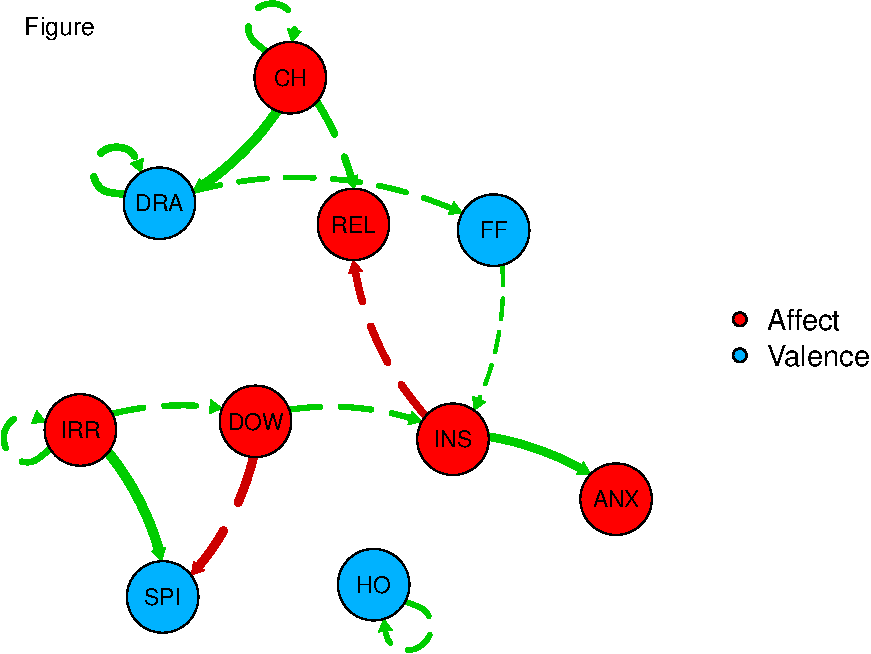
\includegraphics{networkTutorial_files/figure-latex/example1-1.pdf}
\caption{}
\end{figure}

\subsection{Indices of centrality}\label{indices-of-centrality}

To better unbderstand the role of the variables in the network several
statistics for a network have been developped, which are called indices
of centrality.

\subsection{Note}\label{note}

We used R (Version 3.5.1; R Core Team, 2018) and the R-packages
\emph{lagnetw} (Version 0.0.1; Verboon, 2019), and \emph{papaja}
(Version 0.1.0.9842; Aust \& Barth, 2018) for all our analyses.

\newpage

\section{References}\label{references}

\begingroup
\setlength{\parindent}{-0.5in} \setlength{\leftskip}{0.5in}

\hypertarget{refs}{}
\hypertarget{ref-R-papaja}{}
Aust, F., \& Barth, M. (2018). \emph{papaja: Create APA manuscripts with
R Markdown}. Retrieved from \url{https://github.com/crsh/papaja}

\hypertarget{ref-Bringmann2018a}{}
Bringmann, L., \& Eronen, M. (2018). Don't blame the model:
Reconsidering the network approach to psychopathology.
\emph{Psychological Review}, \emph{125}(4), 606--615.
doi:\href{https://doi.org/10.1037/rev0000108}{10.1037/rev0000108}

\hypertarget{ref-Costantini2015}{}
Costantini, G., Epskamp, S., Borsboom, D., Perugini, M., Mõttus, R.,
Waldorp, L. J., \& Cramer, A. O. (2015). State of the aRt personality
research: A tutorial on network analysis of personality data in R.
\emph{Journal of Research in Personality}, \emph{54}, 13--29.
doi:\href{https://doi.org/10.1016/j.jrp.2014.07.003}{10.1016/j.jrp.2014.07.003}

\hypertarget{ref-Epskamp2018}{}
Epskamp, S., Borsboom, D., \& Fried, E. I. (2018). Estimating
psychological networks and their accuracy: A tutorial paper.
\emph{Behavior Research Methods}, \emph{50}(1), 195--212.
doi:\href{https://doi.org/10.3758/s13428-017-0862-1}{10.3758/s13428-017-0862-1}

\hypertarget{ref-R-base}{}
R Core Team. (2018). \emph{R: A language and environment for statistical
computing}. Vienna, Austria: R Foundation for Statistical Computing.
Retrieved from \url{https://www.R-project.org/}

\hypertarget{ref-R-lagnetw}{}
Verboon, P. (2019). \emph{Lagnetw: Lagged networks for esm data}.

\endgroup


\end{document}
